\chapter{Implementation}\label{chap:Implementation}

We implemented the entire visualization pipeline on a Mac OS X server. The implementation consists of an R script as back-end, a Perl CGI script as API, and an HTML/JavaScript web page as user interface.

The R script, \emph{coloring.R}, takes the pair-wise similarity score file as input, performs multidimensional scaling and color optimization, sorts sequences, and output colors and sequence information into two tab-separated files, \emph{colors.tsv} and \emph{seqinfo.tsv}. The front-end web page takes an alignment ID as parameter and sends it to the API. The Perl CGI script parses the color file and sequence information file, along with the FASTA-format alignment file, and sends them back to front-end in JSON format \cite{crockford2006application}. The front-end uses JavaScript to generate the alignment matrix and render it with colors and symbol letters.

\section{R Script}

The script \emph{coloring.R} begins by reading three arguments from command-line calls: score file name, colors file name, and sequence information file name. The first file is for input and the latter two are for output. An example of calling this script on UNIX operating system is given below.
\begin{verbatim}
  Rscript coloring.R data/score.tsv data/colors.tsv data/seqinfo.tsv
\end{verbatim}

The file \emph{score.tsv} contains four columns separated by tabs: column number, first row number, second row number, and similarity score between these two rows in this column. The row and column numbers start from 1, and the similarity score values range from 0 to 1. Figure \ref{fig:score.tsv} shows a few example lines in a \emph{score.tsv} file.
\begin{figure}[hb]
\begin{quote}
\begin{verbatim}
  #COL_NUMBER   #ROW_NUMBER_1   #ROW_NUMBER_2   #RES_PAIR_HIT/NALT
  1             1               2               1.000000
  1             1               6               0.933333
  1             1               10              0.866667
  1             2               6               0.933333
  1             2               10              0.866667
  1             6               10              0.133333
  2             1               6               1.000000
  2             1               10              1.000000
  2             6               10              1.000000
\end{verbatim}
\end{quote}
\caption[Example of Similarity Score File]{An example of similarity score file \emph{score.tsv}, showing the format of the file. The four columns are: column number, the first row number, the second row number, score value.}\label{fig:score.tsv}
\end{figure}

The script \emph{coloring.R} consists of four parts. The first part reads the input file, performs multidimensional scaling and create color for each symbol in the CIE LCH space. The second part rotates and flips color hues and optimize the penalty function. The third part sorts the sequences by their average hues and calculates each sequence’s average RGB color. The last part outputs the symbol colors and sequence information into corresponding files.

The color output file, \emph{colors.tsv}, has five columns separated by tabs: column number, row number, and the symbol color in RGB triplet (red, green, blue) in the range from 0 to 1, which will be converted into hexadecimal format used in the user interface module. The sequence information file seqinfo.tsv also has five columns: row number, average hue from 0 to 360 degrees, and average color in RGB triplet. Figure \ref{fig:color.tsv} shows how a typical \emph{color.tsv} file looks like.
\begin{figure}[hb]
\begin{quote}
\begin{verbatim}
1       1       0.1065524      0.5616907       0.3943046
1       2       0.106256       0.5616652       0.3936842
1       6       0.1065487      0.5616904       0.3942968
1       10      0.1065581      0.5616912       0.3943165
2       1       0.09057406     0.5677889       0.2867890
2       2       0.09057406     0.5677889       0.2867890
2       6       0.09057406     0.5677889       0.2867890
2       10      0.09057406     0.5677889       0.2867890
3       1       0.07634505     0.5664451       0.2581746
3       6       0.1113592      0.570106        0.3250781
3       10      0.07634505     0.5664451       0.2581746
\end{verbatim}
\end{quote}
\caption[Example of Coloring Result File]{An example of coloring result file \emph{color.tsv}, showing the format of the file. The five columns are (from left to right): row number, average hue, red, green and blue.}\label{fig:color.tsv}
\end{figure}

\section{API}

A Perl CGI script, \emph{api.pl}, and a Perl package \emph{Mavis::API} act as the API between the R back-end and HTML/JavaScript front-end. The Perl CGI \emph{api.pl} takes two parameters from HTTP requests, \emph{action} and \emph{id}. The default action is \emph{alignment}, meaning the alignment information, including sequences, colors, average colors and order of sequences, should be returned. In this action, an additional \emph{id} parameter is expected as the alignment ID. Another available action is \emph{list}, which requests a list of all existing alignment IDs.

The API returns the query result to the web page in JSON (JavaScript Object Notation) format, which is a lightweight text-based data-interchange standard. JSON is derived from a subset of JavaScript syntax and can be easily parsed in JavaScript as well as many other languages, like Perl. We included the Perl JSON 2.51 module to provide JSON encoding/decoding ability to our API \cite{crockford2006application}.

Figure \ref{fig:api-res} is an example of the API response in JSON format:
\begin{figure}[hb]
\begin{quote}
\begin{verbatim}
  { "status"    : 1,
    "id"        : "demo",
    "colors"    : [ ["#666","#666","#666","#666"],
                    ["#665","#667","#667","#665"]],
    "sequences" : [ {"name":"Seq02", "color":"#26e", "seq":"DEMO"},
                    {"name":"Seq01", "color":"#26e", "seq":"DEMO"}]
  }
\end{verbatim}
\end{quote}
\caption[Example of API Response in JSON Format]{An example of Mavis API response in JSON format.}\label{fig:api-res}
\end{figure}

\section{User Interfaces}

We implement an web interface with HTML and JavaScript to send API requests and draw visualization graphs. The JavaScript code dynamically communicates with API, creates an HTML table, and fills in colors and symbols. This part is simplified by jQuery, which is a popular cross-platform JavaScript library that abstracts complicated DOM selection, CSS manipulation and Ajax effects.

\begin{landscape}
\begin{figure}[p]
\center{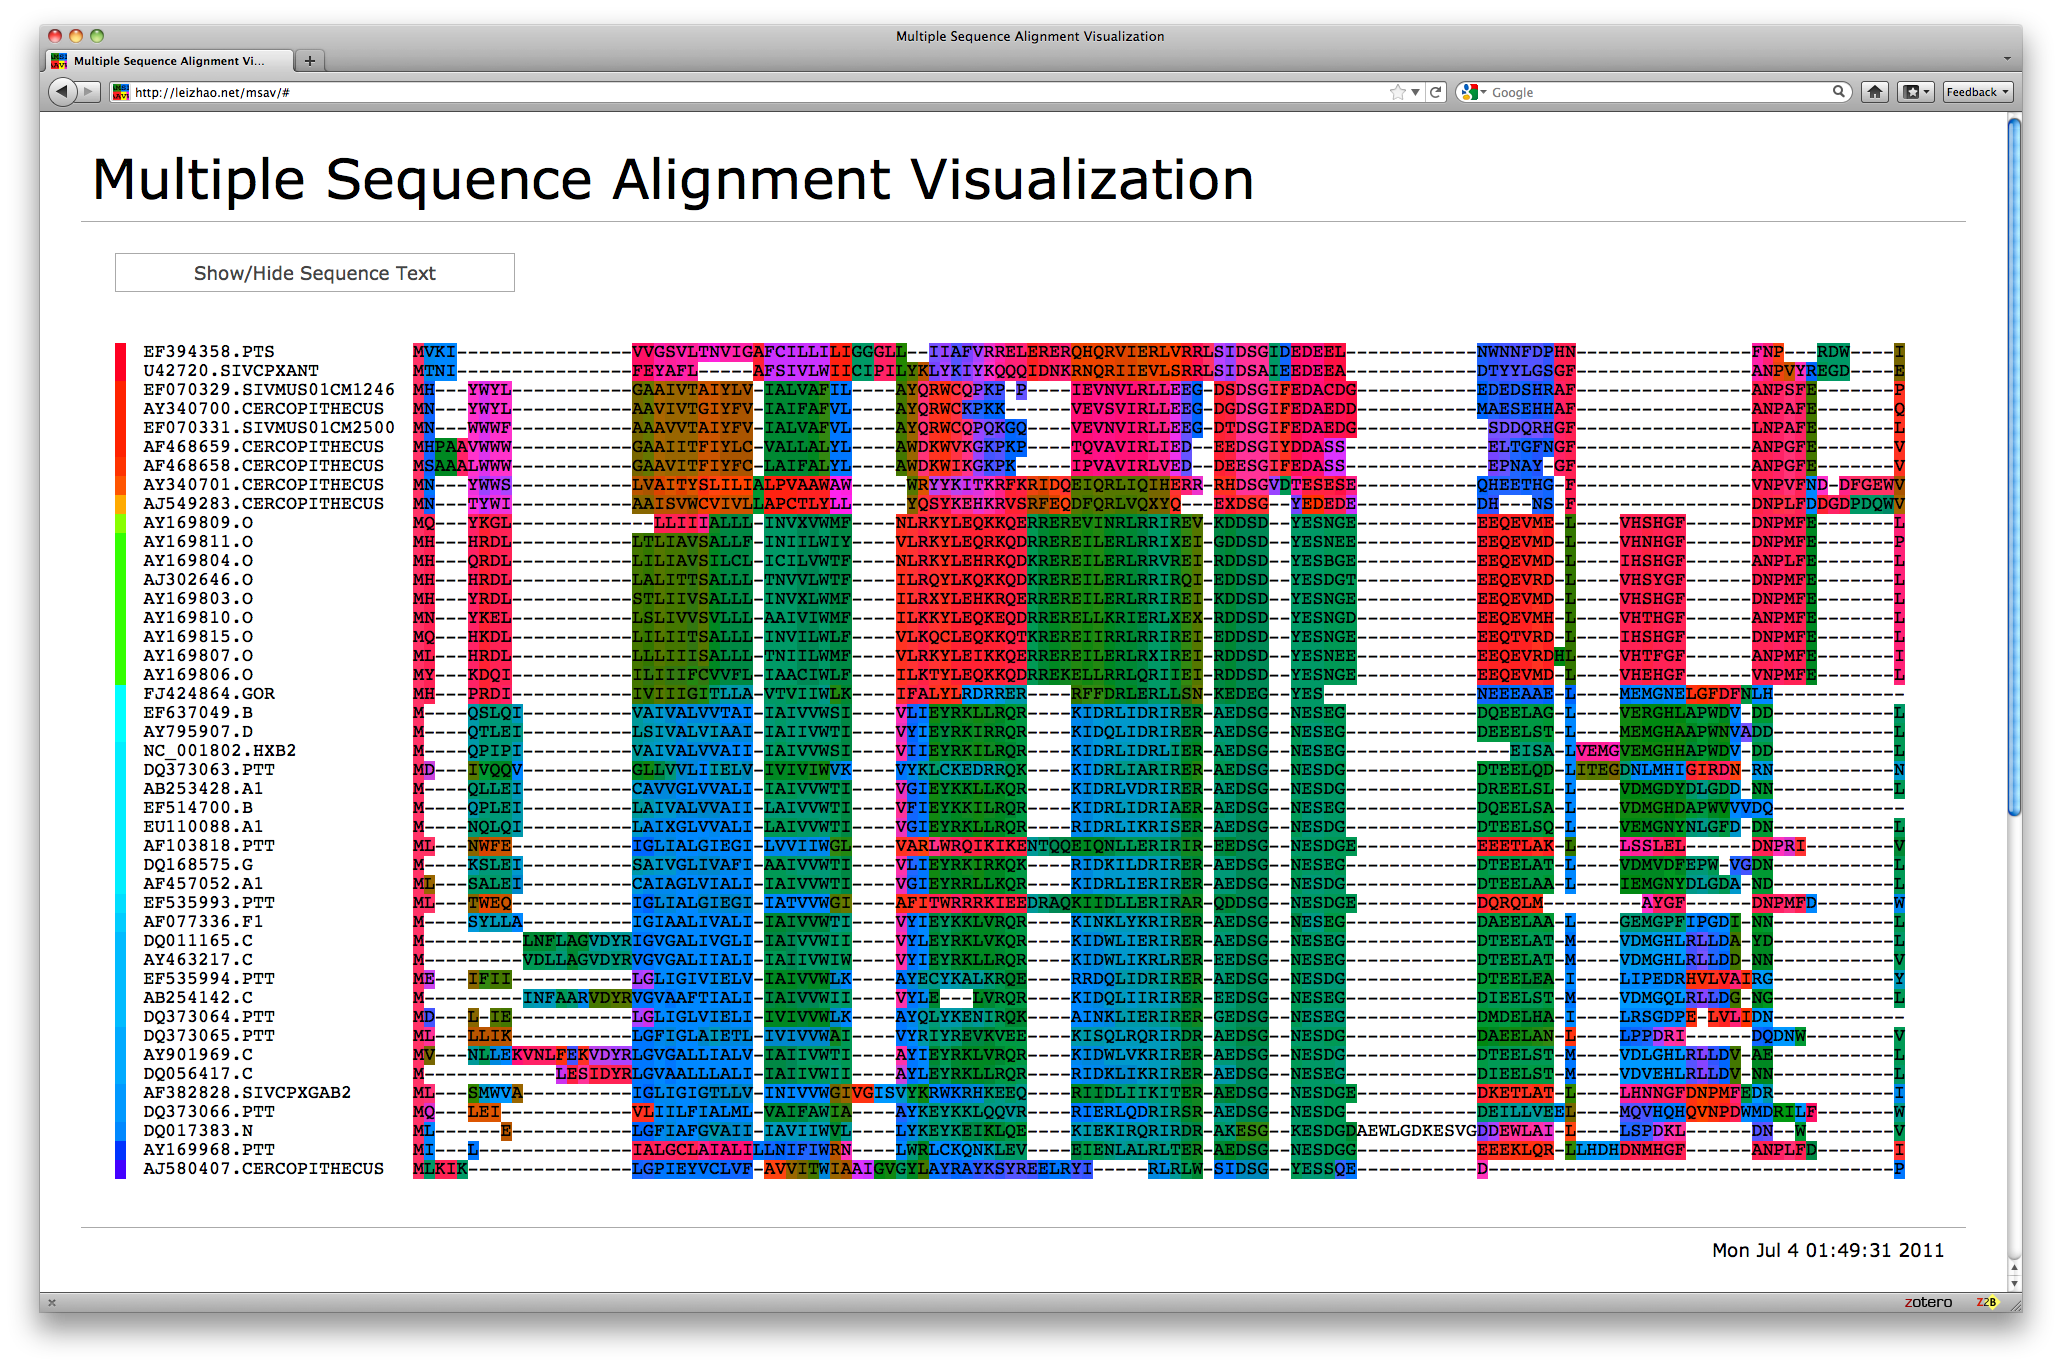
\includegraphics[height=0.83\textwidth]{figures/chap4_mavis.png}}
\caption[MSA Rendered by Mavis in Web Browser]{An MSA rendered by Mavis in Firefox 5.}\label{fig:chap4_mavis}
\end{figure}
\end{landscape}

\section{Design Principles}